\documentclass{bioinfo}
\copyrightyear{2015} \pubyear{2015}
\usepackage{graphicx}
\usepackage{booktabs}
\usepackage{colortbl, xcolor}
\access{Advance Access Publication Date: Day Month Year}
\appnotes{Manuscript Category}

\begin{document}
\firstpage{1}

\subtitle{Subject Section}

\title[Prediction of amyloidogenicity based on the n-gram analysis]{Prediction of amyloidogenicity based on the n-gram analysis}
\author[Sample \textit{et~al}.]{Micha\l{} Burdukiewicz$^{\text{\sfb 1,*}}$, Piotr Sobczyk\,$^{\text{\sfb 2}}$, Pawe\l{} Mackiewicz$^{\text{\sfb 1}}$ and Ma\l{}gorzata Kotulska\,$^{\text{\sfb 3,}*}$}
\address{$^{\text{\sf 1}}$University of Wroc\l{}aw, Department of Genomics,
$^{\text{\sf 2}}$Wroc\l{}aw University of Technology, Department of Mathematics and 
$^{\text{\sf 3}}$Wroc\l{}aw University of Technology, Department of Biomedical Engineering, Faculty of Fundamental Problems of Technology
}

\corresp{$^\ast$To whom correspondence should be addressed.}

\history{Received on XXXXX; revised on XXXXX; accepted on XXXXX}

\editor{Associate Editor: XXXXXXX}

\abstract{\textbf{Motivation:} Text Text Text Text Text Text Text Text Text Text Text Text Text
Text Text Text Text Text Text Text Text Text Text Text Text Text Text Text Text Text Text Text
Text Text Text Text Text Text Text Text Text Text Text Text Text Text Text Text Text Text Text
Text Text Text Text Text Text
Text Text Text Text Text.\\
\textbf{Results:} Text  Text Text Text Text Text Text Text Text Text  Text Text Text Text Text vvv
% * <michalburdukiewicz@gmail.com> 2016-02-23T09:35:35.738Z:
%
% ^.
Text Text Text Text Text Text Text Text Text Text Text Text Text  Text Text Text Text Text Text\\
\textbf{Availability:} Text  Text Text Text Text Text Text Text Text Text  Text Text Text Text
Text Text Text Text Text Text Text Text Text Text Text Text Text Text  Text\\
\textbf{Contact:} \href{name@bio.com}{name@bio.com}\\
\textbf{Supplementary information:} Supplementary data are available at \textit{Bioinformatics}
online.}

\maketitle

\section{Introduction}


%\enlargethispage{12pt}

\section{Approach}



\begin{methods}
\section{Methods}

\subsection{Data set}

The data used in the study was extracted from AmyLoad data 
base~\citep{wozniak_amyload:_2015}. Aside from eight sequences shorter than five 
residues that were removed from the final data set, we obtained 418 
amyloidogenic sequences and 1039 non-amyloidogenic sequences (1457 peptides in 
total).

  Sequences shorter than 6 amino acids and longer than 25 amino acids were 
removed from data set. The former were too short to be processed in the devised 
analysis framework and the latter were too diversified and rare, preventing the 
proper analysis.

  The final data set contains 397 amyloidogenic and 1033 non-amyloidogenic 
sequences (1430 peptides in total).

\subsection{Encodings of amino acids}

The amyloidogenicity of given peptide may not depend on the exact sequence of 
amino acids, but on its more general properties. To verify this hypothesis, we 
created 524 284 reduced amino acid alphabets (encodings) with different lengths 
(from three to six letters) using Ward's 
clusterization~\citep{jr_hierarchical_1963} on the selected physicochemical 
properties from AAIndex database~\citep{kawashima_aaindex:_2008}. We handpicked 
several measures belonging to more general categories important in process of 
amyloidogenicity as size, hydrophobicity, solvent surface area, frequency in 
$\beta$-sheets and contactivity. As the rule of thumb, we limited ourselves to 
properties introduced after 1980 when, thanks to the technological advancements, 
the measurements were more accurate.

  The majority of encodings had at least one duplicate. In such case, only the 
single representative was included in the cross-validation. After filtering 
duplicates, we obtained 18 535 unique encodings.

\begin{table*}[bth]
\centering
\begin{tabular}{ll}
  \hline
Category & Property \\ 
  \hline
  Contactivity & Average flexibility indices \citep{bhaskaran_positional_1988} \\ 
  Contactivity & 14 A contact number \citep{nishikawa_radial_1986} \\ 
  Contactivity & Accessible surface area \citep{radzicka_comparing_1988} \\ 
    Contactivity & Buriability \citep{zhou_quantifying_2004} \\ 
  Contactivity & Values of Wc in proteins from class Beta, cutoff 12 A, separation 5 \citep{wozniak_characteristics_2014} \\ 
  Contactivity & Values of Wc in proteins from class Beta, cutoff 12 A, separation 15 \citep{wozniak_characteristics_2014} \\ 
  $\beta$-frequency & Average relative probability of inner beta-sheet \citep{kanehisa_local_1980} \\ 
  $\beta$-frequency & Relative frequency in beta-sheet \citep{prabhakaran_distribution_1990} \\ 
  $\beta$-frequency & Thermodynamic beta sheet propensity \citep{kim_thermodynamic_1993} \\ 
  Hydrophobicity & Hydrophobicity index \citep{argos_structural_1982} \\ 
  Hydrophobicity & Optimal matching hydrophobicity \citep{sweet_correlation_1983} \\ 
  Hydrophobicity & Hydrophobicity-related index \citep{kidera_statistical_1985} \\ 
  Hydrophobicity & Scaled side chain hydrophobicity values \citep{black_development_1991} \\ 
  Polarity & Polarizability parameter \citep{charton_structural_1982} \\ 
  Polarity & Mean polarity \citep{radzicka_comparing_1988} \\ 
  Size & Average volumes of residues \citep{pontius_deviations_1996} \\ 
  Stability & Side-chain contribution to protein stability (kJ/mol) \citep{takano_new_2001} \\ 
   \hline
\end{tabular}
\caption{Physicochemical properties used in the creation of reduced amino acid alphabets.} 
\end{table*}

  Since highly correlated or, contrarily, uncorrelated measures create very 
similar encodings, we further reduced the number of properties to 17 by 
selecting measures with the absolute value of Pearson's correlation coefficient 
for normalized values larger than 0.95.

\subsection{Training of learners}

\begin{figure*}[!tpb]%figure1
\centerline{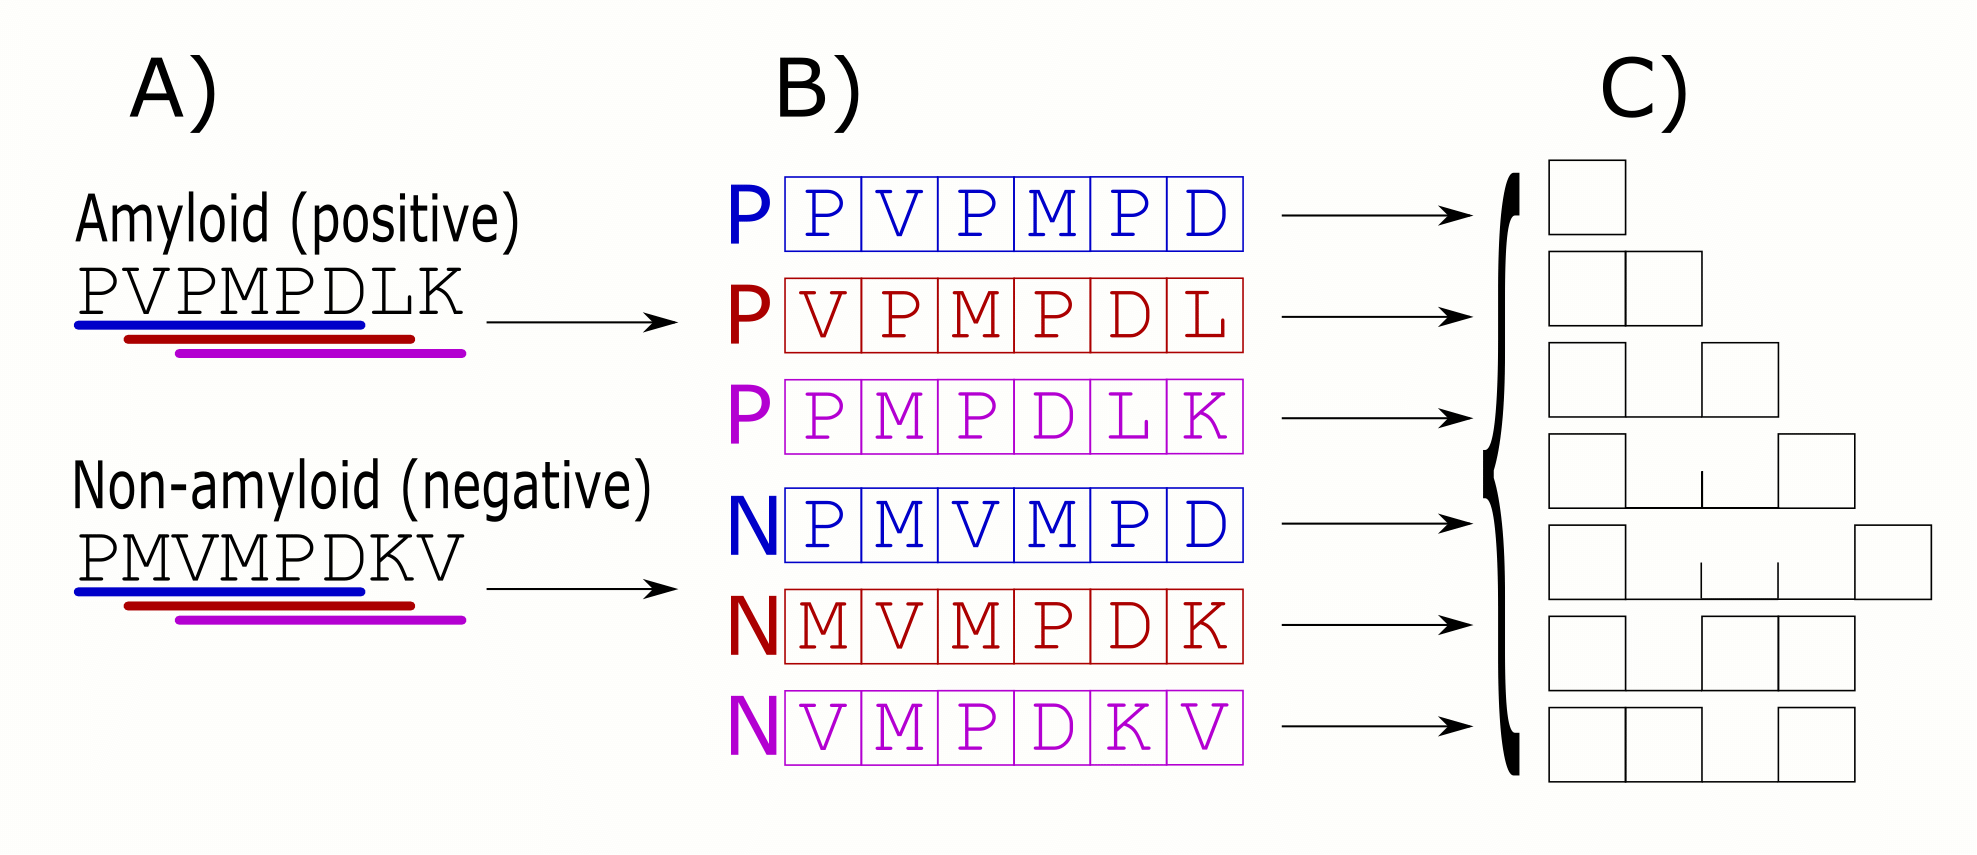
\includegraphics[width=\textwidth]{figures/ngram_scheme.png}}
  \caption{The scheme of n-gram extraction. A) Input data - peptides with a 
known amyloidogenicity status. B) Each peptide sequence was divided into 
overlapping hexamers. The amyloidogenicity status of a source sequence was used 
as the amyloidogenicity status of a derived hexamer. C) From each hexamer we 
extracted continuous 1-, 2- and 3-grams. We selected also gapped 2-grams with 
the length of gap equal from 1 to 3 residues and gapped 3-grams with a single 
gap between the first and the second or the second and the third element of the 
n-gram.}
\label{fig:ngram_scheme}
\end{figure*}

During the training phase, we extracted overlapping hexamers from each sequence. 
Each hexamer was tagged with the same etiquette (amyloid/nonamyloid) as the 
original peptide. For example, the sequence of length 6 residues yields only one 
hexamer and the sequence of 8 residues yields 3 hexamers 
(Fig.~\ref{fig:ngram_scheme} A and B).  Assuming that in longer amyloids only a 
short part of the sequence is responsible for amyloidogenicity, our method might 
results in many false positives in the training data set. To evade this problem, 
we restricted the maximum length of peptides in training data set to fifteen 
amino acids to easy the extraction of probable hot-spots.

  From each hexamer we extracted n-grams of the following length: 1, 2 and 3. In 
the case of 2- and 3-grams, we separately counted both gapped and continuous 
n-grams. For 2-grams we counted n-grams with gaps of lengths from 1 to 3 and for 
3-grams with a single gap between the first and the second or the second and the 
third element (see Fig.~\ref{fig:ngram_scheme}).

  The study the length of amyloidogenicity signal, we trained three 
classifiers for each encoding on the sequences of different length. We 
considered separately six-residue sequences, shorter of equal to ten residues 
and shorter or equal to fifteen residues.

  All n-grams extracted from the hexamers in the training data set were filtered 
using described below Quick Permutation Test with the information gain (mutual 
information) as the criterion of the importance of a specific n-gram. In the 
next step, we used n-grams with the p-value smaller than 0.05 to build a random 
forest~\citep{breiman_random_2001} classifier using ranger \textbf{R} 
package~\citep{wright_ranger:_2015}. 

  Furthermore, we repeated the procedure described above on two typical reduced 
alphabets of amino acids derived from the literature to check if the process of 
amyloidogenicity does require nonstandard groupings of amino acids. We also 
added the full amino acid alphabet to assess the advantages of the amino acid 
encoding.

\subsection{Quick Permutation Test (QuiPT)}

In this section we outline how to filter n-gram features without performing huge number of permutations. 
Let us consider the contingency table for target $y$ and feature $x$:

\begin{center}
\begin{tabular}{ | c || c | c | }
  \hline			
  target / feature & 1 & 0 \\ \hline
 1 & $n_{1,1}$ & $n_{1,0}$ \\
 0 & $n_{0,1}$ & $n_{0,0}$ \\
  \hline  
\end{tabular} 
\end{center}

Under the hypothesis that $x$ an $y$ are independent, the probability of such a contingency  table 
is given by the multinomial distribution. In the permutation test we simply reshuffle 
feature and target labels, but the total number of positives in both of them
is fixed. When we impose this constraint on the multinomial distribution then
it depends only on $n_{1,1}$ and is fairly easy to compute.
Observe also, that $n_{1,1}$ is from range $[0,min(n_{\cdot, 1}, n_{1, \cdot})]$.
After computing Information Gain for each possible value of $n_{1,1}$, we get
distribution of Information Gain under hypothesis that target and feature
are independent. We reject null hypothesis when Information Gain is big.

 Having the analytical formula for the distribution, allows us to perform permutation test much quicker. 
Furthermore, we get exact quantiles even for extreme tails of the distribution,
which is not guaranteed by random permutations. 
In fact, imagine performing test with $\alpha=10^{-8}$, which is
not an uncommon value, i.e. when we adjust for multiple testing.
Even for huge number of permutations like $m=10^8$, standard deviation of quantile estimate 
in permutation test, $\frac{p(1-p)}{m}$, is roughly equal to $\alpha$ itself.

 In the context of k-mer data we can speed up our algorithm even further. Note that
since target $y$ is common for testing all k-mer features, test statistics depends only on
$n_{\cdot, 1}$ -- the number of positive cases in a feature. 
Though we test millions of features, there are just few distributions
that we need to compute, as usually number of positives in k-mer feature is small. 
We take advantage of this fact and we compute quantiles for just a handful of distributions.
Therefore complexity of our algorithm is roughly equal $O(n\cdot p)$.

Lastly, let us point out that QuiPT is very similar for Fisher's exact test.
From the derivation provided in i.e.~\citep{lehmann2008testing}, it becomes obvious that
QuiPT is a heuristics for an unsolved problem of a two-tailed Fisher's exact test.
In this heuristics, extremity of a contingency table, is defined by the amount of 
Information Gain it provides.

\subsection{Cross-validation and selection of the best-performing encoding}

The ability to correctly predict amyloidogenicity was assessed during the 
five-fold cross-validation. Since the data set was very heterogeneous, we 
repeated the cross-validation fifteen times for each classifier to obtain more 
precise estimates of performance measures for each classifier. 

  To evaluate if our classifiers are able to use decision rules extracted from 
sequences of given length to correctly classify longer or shorter sequences, we 
calculate performance measures separately for four ranges of lengths of 
sequences: 6, 7-10, 11-15 and 16-25. The number of sequences from the given 
length range was roughly comparable between folds of cross-validation.
  
  To choose the most adequate reduced amino acid alphabet, we ranked the values 
of AUC (with rank 1 for the best AUC, rank 2 for the second best AUC and so on) 
for each range of sequence length in the testing data set. The encoding with 
the lowest sum of ranks from all sequence length categories was selected as 
the best one. For this encoding, we choose the range of peptides length in the 
training set providing the best AUC in cross-validation.

\subsection{Encoding distance}
The encoding distance is a measure defining the similarity between two 
encodings. It has zero value for identical encodings and grows with the 
diffences between encodings. It was introduced to verify if the reduced 
alphabets very similar to the best-performing encoding will also have good 
prediction performance.

  We define the encoding distance as the minimum number of amino acids that 
have to be moved between subgroups of encoding to make \textit{a} identical to 
\textit{b} (the order of subgroups in the encoding and amino acids in a group 
is unimportant). This measure is further scaled by a factor reflecting how 
much moving amino acids between groups altered mean group properties. 

To compute the scale factor $s$ for the encoding distance between 
encoding \textit{a} with $n$ subgroups and encoding \textit{b} with $m$ 
subgroups we firstly calculate $p_i$ and $p_j$, mean values of physicochemical 
properties of all amino acids separately for each subgroup. The factor between 
$a$ and $b$ is equal to: 

$$
s_{ab} = \sum^n_{i = 1}  \left( \min_{j=1,\dots,m} \left(\sqrt{\sum^l p_{i}^2} 
- \sqrt{\sum^l p_{j}^2} \right) \right)
$$
 
where $l$ is equal to the number of physicochemical properties of concern.

\subsection{Benchmark of AmyloGram}

The best-performing reduced amino acid alphabet chosen during the 
cross-validation was later used to train AmyloGram, n-gram based predictor of 
amyloidogenicity.

  We used \textit{pep424} data set~\citep{walsh_pasta_2014} to compare the 
performance of AmyloGram and other predictors of amyloidogenicity. Since the 
model of AmyloGram does not covers peptides shorter than five amino acids, we 
removed them from the total benchmark data set. It should not affect the 
comparison as only five sequences were eliminated (around 1\% of the original 
data set). Additionally, we also benchmarked three predictors learned on the 
n-grams extracted from sequences of different length ranges without any amino 
acid encoding.

  All benchmarked classifiers were trained on sequences used during the 
cross-validation. Since some peptides were common for both \textit{pep424} and 
AmyLoad, we removed them from the training data set. After purification, the 
learning data set had 269 positive sequences and 746 negative sequences longer 
than five residues and shorter than fifteen residues. Aside from the 
preparation of the training data, we exactly repeated the procedure of n-gram 
extraction as described above (see Fig.~\ref{fig:ngram_scheme}). 

\end{methods}

\section{Results and discussion}

\subsection{Selection of the best-performing encoding}

\begin{figure*}[!tpb]
\centerline{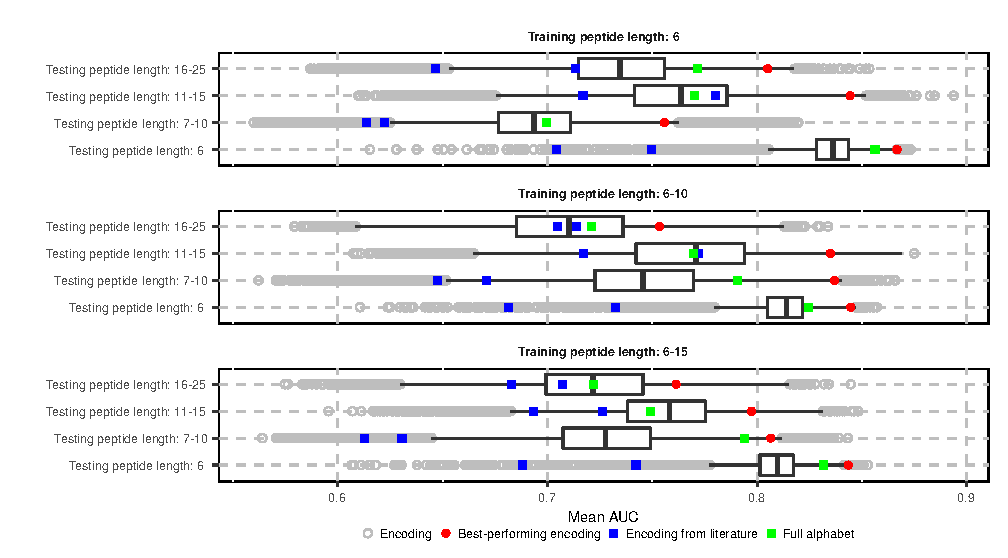
\includegraphics{figures/AUC_boxplot.eps}}
\caption{Distribution of AUC values of different reduced amino acid alphabets 
for different lengths of sequences in the training and testing data sets.
%Red circle: classifier employing best encoding of amino acid. Green square: 
%classifier using full amino acid alphabet. Blue square: classifiers employing 
%encodings from literature.
}\label{fig:AUC_boxplot} 
\end{figure*}

\begin{figure*}[!tpb]
\centerline{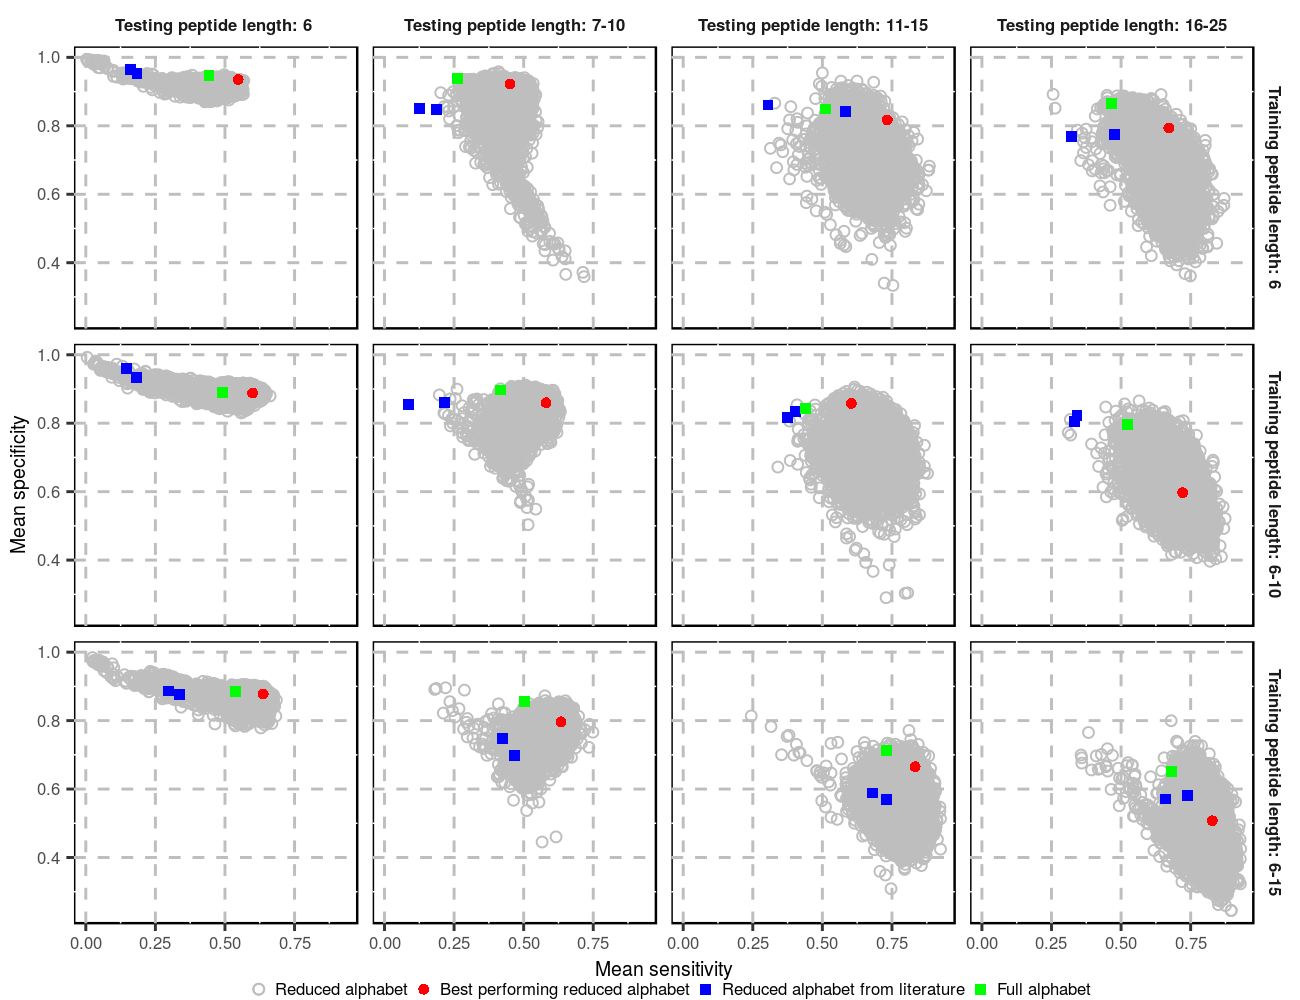
\includegraphics{figures/sesp_plot.png}}
\caption{Sensitivity and specificity of classifiers in cross-validation for 
different lengths of sequences in the training and testing data sets.
%Red 
%circle: classifier employing best encoding of amino acid. Green square: 
%classifier using full amino acid alphabet. Blue square: classifiers employing 
%encodings from literature. 
The classifier based on the best-performing encoding always have 
good specificity and sensitivity.}\label{fig:sesp_plot}
\end{figure*}

The selected encoding performed better than other reduced alphabets 
considering all sequence length ranges in training and testing data set. It has 
the AUC always in the fourth quartile (Fig.~\ref{fig:AUC_boxplot}). For the 
best-performing encoding the most problematic was correct prediction of the 
amyloidogenicity in the longest peptides 16-25 not when learned on very short 
sequences, but longer ones (6-10 and 6-15). Such behavior was typical for most 
of the analyzed encodings.

  The highest values of AUC the chosen encoding reaches in the relatively the 
simplest cases of predicting amyloidogenicity of the shortest sequences (6 
residues). Of course, the decision rules were the easiest to extract when also 
the learning set has only sequences of the same lengths, but results were quite 
comparable even if the training set contained longer sequences. Also in this 
situation, majority of reduced amino acid alphabets behaved like the selected 
encoding and also have higher AUC than in other scenarios.

  Considering only the AUC value, the most problematic testing data were 
sequences longer than 15 amino acids. Surprisingly, the classifiers trained on 
the shortest sequences available (six residues) were performing the best. That 
might indicate that our n-gram approach extracts the important features the 
better, the shorter are sequences in training data set. For example, in the 
amyloidogenic peptide of length 15, only a very specific region of residues 
might be responsible for the creation of harmful aggregates. In this case, when 
in our framework overlapping n-grams are extracted, only part of them may carry 
the true signal of amyloidogenicity, but all are marked as amyloids. 
Despite this problem, the overall prediction of classifiers learned on the long 
sequences was still adequate, with the median values of AUC higher than 0.7 for 
every testing set. 

  In addition to the high AUC, the best encoding has also very good sensitivity 
and specificity regardless of the length of sequences in training and testing 
set (Fig.~\ref{fig:sesp_plot}). The classifiers trained on the peptides of 
length 6 tend to have the best specificity, while predictors learned on the long 
sequences have the best sensitivity. Albeit the classifiers trained on 
six-residue-long sequences have generally better AUC, training on 
the sequences ranging from six to ten residues seem to yield most balanced 
classifiers with optimal sensitivity and specificity.

  We also evaluated classifiers based on the full amino acid alphabet. In most 
cases they also places in the fourth quartile considering their AUC value 
(Fig.~\ref{fig:AUC_boxplot}). Nevertheless, they never predict amyloidogenicity 
better than the selected encoding. It suggests that despite the predictive power 
of n-grams based on full alphabet, the encoding allows better generalization of 
the prediction rules and in the consequence better performance.

  Similarly to the best-performing encoding, the sensitivity of classifiers 
based on the full amino acid alphabet seems to decrease with the length of 
sequences in the training data set (Fig.~\ref{fig:sesp_plot}). Furthermore, 
these classifiers seem to always have one of the worst sensitivities among all 
analyzed predictors, especially when tested on longer amyloids. It means that 
using the full amino acid alphabet it easier to point the non-amyloidogenic 
sequences instead of recognizing amyloids.

  The encodings found in the literature performs substantively worse than other 
analyzed amino acid alphabets in all categories. It indicates that classical 
divisions of amino acids do not create groups suitable for the recognition of 
amyloids. This observation is well-supported by the specificity-sensitivity 
plot (Fig.~\ref{fig:sesp_plot}), where classifiers trained with this encodings 
of amino acids groups with the worst performers.

\subsection{The best-performing encoding and important n-grams}

\begin{figure}[!tpb]
\centerline{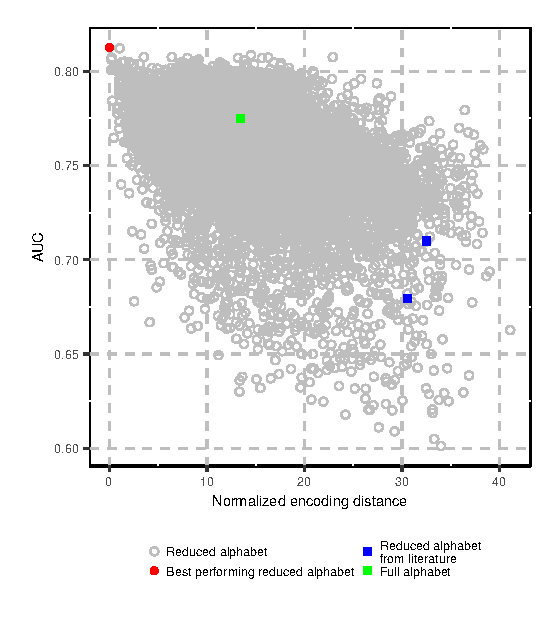
\includegraphics{figures/ed_AUC.eps}}
\caption{The encoding distance and AUC of reduced alphabets studied in the 
cross-validation. 
%Red circle: classifier employing best encoding of amino acid. Green square: 
%classifier using full amino acid alphabet. Blue square: classifiers employing 
%encodings from literature. 
Classifiers having the smallest encoding distance to the best classifier have 
the highest AUC.}\label{fig:ed_AUC}
\end{figure}

% latex table generated in R 3.2.3 by xtable 1.8-2 package
% Tue Mar  8 14:20:53 2016
\begin{table}[ht]
\centering
\caption{The best-performing encoding.} 
\label{tab:best_enc}
\begin{tabular}{cl}
\toprule
Subgroup ID & Amino acids \\ 
\midrule
  1 & G \\ 
\rowcolor[gray]{0.85}  2 & K, P, R \\ 
3 & I, L, V \\ 
\rowcolor[gray]{0.85}  4 & F, W, Y \\ 
5 & A, C, H, M \\ 
\rowcolor[gray]{0.85}  6 & D, E, N, Q, S, T \\ 
\bottomrule
\end{tabular}
\end{table}


\begin{figure}[!tpb]
\centerline{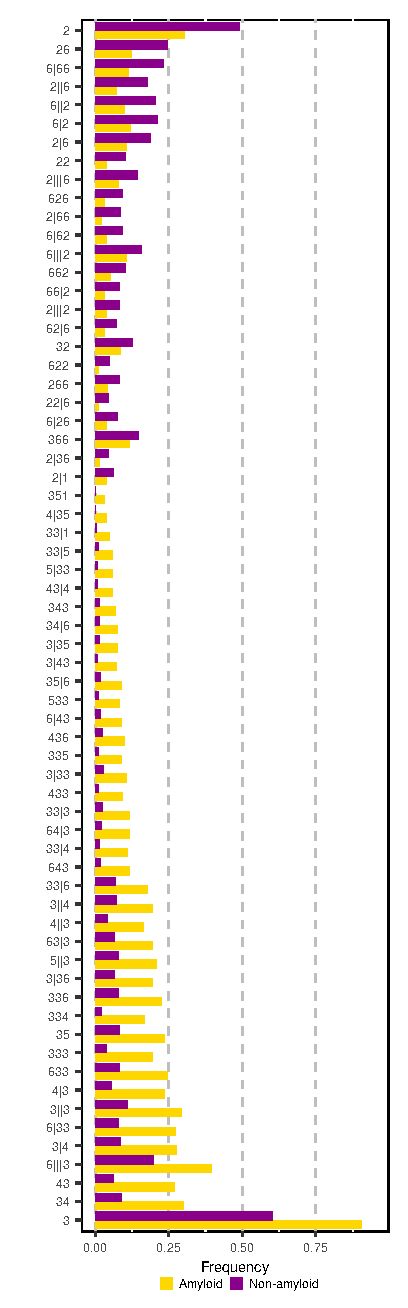
\includegraphics{figures/ngrams.eps}}
\caption{Important n-grams. }\label{fig:ngrams}
\end{figure}

The reduced amino acid alphabet chosen during the analysis has six subgroups 
(Tab.~\ref{tab:best_enc}). Two subgroups, 3 and 4 contain mostly hydrophobic 
amino acids, while 1 and 4 are mostly hydrophilic. In addition to this, subgroup 
1 and 4 have amino acid with the highest average flexibility. The least flexible 
amino acids are in subgroup 5. The most polarizable amino acids belong to 
subgroup 4, while the lowest polarizability is typical for glycine, the 
only amino acid in subgroup 1. The glycine has also the highest thermodynamic 
beta sheet propensity, which has the lowest values for subgroups 3 and 4.

  Identical reduced amino acid alphabets were created through ten other 
combinations of physicochemical properties. Only four features appeared in all 
eleven combinations: hydrophobicity index~\citep{argos_structural_1982}, average 
flexibility indices~\citep{bhaskaran_positional_1988}, polarizability 
parameter~\citep{charton_structural_1982} and thermodynamic beta sheet 
propensity~\citep{kim_thermodynamic_1993}.

  We calculated encoding distances between the best-performing reduced amino 
acid alphabet and other encodings (Fig.~\ref{fig:ed_AUC}). To compute the scale 
factor, we used described above features common for all encodings identical to 
the best-performing one. The value of AUC is significantly lower for more 
distant encodings ($-0.4370$ Pearson's correlation coefficient, p-value smaller 
than $2.2 \times 10^{-16}$). Such relationship between AUC and encoding distance 
confirms that only reduced alphabets sufficiently similar to the best-performing 
encoding are able to remove unnecessary diversity while preserving information 
important for recognition of amyloids.



  We discovered that 65 n-grams have p-values smaller than 0.05 in the every 
fold of repetitions of cross-validation regardless of the training set. 

  


\subsection{Benchmark of AmyloGram}

The benchmark covered Amylogram as well as two best-performing peer-reviewed 
predictors of amyloidogenicity (PASTA2~\citep{walsh_pasta_2014} and 
FoldAmyloid~\citep{garbuzynskiy_foldamyloid:_2010}). We analyzed Area Under the 
Curve (AUC), Matthew's Correlation Coefficient (MCC), Sensitivity and 
Specificity (see Tab.~\ref{tab:bench_summary}).
    
  Interestingly, the n-gram extraction method was efficient enough to produce 
classifiers able to outperformed published methods. Two of three n-gram based 
classifiers trained on the full alphabet have AUC higher than PASTA2 and all 
three were more successful than FoldAmyloid. They also maintained they high 
Specificity as seen previously during cross-validation.
    
  Although the proposed n-gram extraction creates efficient classifiers, the 
encoding of amino acids further increases the prediction of amyloidogenicity. 
AmyloGram has the highest AUC, MCC and Sensitivity among all tested classifiers. 
Is has lower specificity than two classifiers trained on the full alphabet, but 
still outperforms other published method in this category. It is important to 
highlight that AmyloGram is the most balanced of analyzed classifiers, having 
the best Specificity/Sensitivity balance, as indicated by the value of MCC.

% latex table generated in R 3.2.3 by xtable 1.8-2 package
% Tue Mar  8 14:17:55 2016
\begin{table}[ht]
\centering
\caption{Results of benchmark on \textit{pep424} data set for AmyloGram, 
PASTA2, FoldAmyloid and random forest predictor learned on n-grams extracted 
without any amino acid encoding from the sequences of the length specified in 
the brackets.} 
\label{tab:bench_summary}
\begin{tabular}{ccccc}
  \toprule
Classifier & AUC & MCC & Sensitivity & Specificity \\ 
  \midrule
AmyloGram & \textbf{0.8972} & \textbf{0.6307} & \textbf{0.8658} & 0.7889 \\ 
   \rowcolor[gray]{0.85}PASTA2 & 0.8550 & 0.5227 & 0.7987 & 0.7444 \\ 
  FoldAmyloid & 0.7351 & 0.4526 & 0.7517 & 0.7185 \\ 
   \rowcolor[gray]{0.85}full alphabet (6) & 0.8411 & 0.5427 & 0.4966 & 
\textbf{0.9593} \\ 
  full alphabet (6-10) & 0.8581 & 0.5698 & 0.7517 & 0.8259 \\ 
   \rowcolor[gray]{0.85}full alphabet (6-15) & 0.8610 & 0.5490 & 0.8188 & 0.7519 
\\ 
   \bottomrule
\end{tabular}
\end{table}

\section{Conclusion}



\section*{Acknowledgments}

\noindent Calculations have been carried out in Wroclaw Center for Networking 
and Supercomputing (http://www.wcss.pl), grant No. 347.

\section*{Funding}

This research was partially funded by the KNOW Consortium.

\bibliographystyle{natbib}
%\bibliographystyle{achemnat}
%\bibliographystyle{plainnat}
%\bibliographystyle{abbrv}
%\bibliographystyle{bioinformatics}
%
%\bibliographystyle{plain}
%
\bibliography{amyloids}
\end{document}
